\documentclass[11pt,border=6pt]{standalone}
\usepackage{fontspec}
\usepackage{tikz}
\usetikzlibrary{positioning,arrows.meta,calc}
\begin{document}
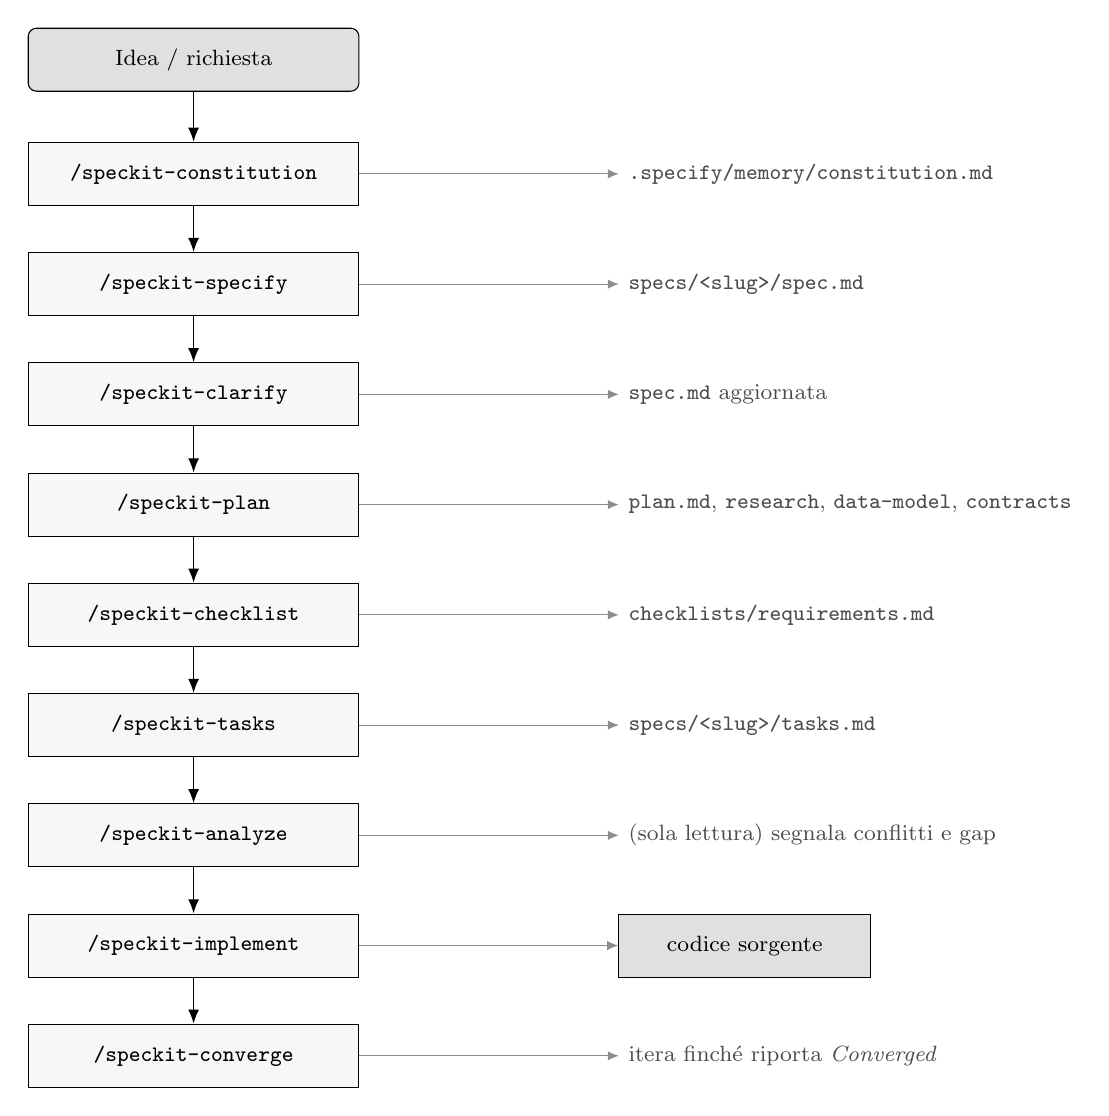
\begin{tikzpicture}[font=\footnotesize,
  cmdbox/.style={draw, minimum width=4.2cm, minimum height=8mm, align=center,
    fill=black!3, font=\footnotesize},
  startbox/.style={draw, rounded corners=3pt, minimum width=4.2cm, minimum height=8mm,
    align=center, fill=black!12, font=\footnotesize},
  resbox/.style={draw, minimum width=3.2cm, minimum height=8mm, align=center,
    fill=black!12, font=\footnotesize},
  artlbl/.style={font=\footnotesize, text=black!70, anchor=west},
  arr/.style={-{Latex[length=1.8mm,width=1.4mm]}, semithick},
  sidearr/.style={-{Latex[length=1.4mm,width=1.2mm]}, black!45}]

  \node[startbox] (idea) at (0,0) {Idea / richiesta};

  \node[cmdbox] (const) at (0,-1.45) {\texttt{/speckit-constitution}};
  \node[artlbl]  (constA) at (5.4,-1.45) {\texttt{.specify/memory/constitution.md}};

  \node[cmdbox] (spec) at (0,-2.85) {\texttt{/speckit-specify}};
  \node[artlbl]  (specA) at (5.4,-2.85) {\texttt{specs/<slug>/spec.md}};

  \node[cmdbox] (clar) at (0,-4.25) {\texttt{/speckit-clarify}};
  \node[artlbl]  (clarA) at (5.4,-4.25) {\texttt{spec.md} aggiornata};

  \node[cmdbox] (plan) at (0,-5.65) {\texttt{/speckit-plan}};
  \node[artlbl]  (planA) at (5.4,-5.65) {\texttt{plan.md}, \texttt{research}, \texttt{data-model}, \texttt{contracts}};

  \node[cmdbox] (check) at (0,-7.05) {\texttt{/speckit-checklist}};
  \node[artlbl]  (checkA) at (5.4,-7.05) {\texttt{checklists/requirements.md}};

  \node[cmdbox] (tasks) at (0,-8.45) {\texttt{/speckit-tasks}};
  \node[artlbl]  (tasksA) at (5.4,-8.45) {\texttt{specs/<slug>/tasks.md}};

  \node[cmdbox] (analyze) at (0,-9.85) {\texttt{/speckit-analyze}};
  \node[artlbl]  (analyzeA) at (5.4,-9.85) {(sola lettura) segnala conflitti e gap};

  \node[cmdbox] (impl) at (0,-11.25) {\texttt{/speckit-implement}};
  \node[resbox]  (implA) at (7.0,-11.25) {codice sorgente};

  \node[cmdbox] (conv) at (0,-12.65) {\texttt{/speckit-converge}};
  \node[artlbl]  (convA) at (5.4,-12.65) {itera finché riporta \emph{Converged}};

  \foreach \a/\b in {idea/const, const/spec, spec/clar, clar/plan, plan/check, check/tasks, tasks/analyze, analyze/impl, impl/conv}
    \draw[arr] (\a.south) -- (\b.north);

  \foreach \a/\b in {const/constA, spec/specA, clar/clarA, plan/planA, check/checkA, tasks/tasksA, analyze/analyzeA, conv/convA}
    \draw[sidearr] (\a.east) -- (\b.west);
  \draw[sidearr] (impl.east) -- (implA.west);
\end{tikzpicture}
\end{document}


